\XtoCBlock{Constant}
\label{block:Constant}
\begin{figure}[H]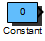
\includegraphics{Constant}\end{figure} 

\begin{XtoCtabular}{Outports}
Out & Constant output\tabularnewline
\hline
\end{XtoCtabular}

\begin{XtoCtabular}{Mask Parameters}
Value & Constant factor\tabularnewline
\hline
\end{XtoCtabular}

\subsubsection*{Description:}
Constant value.

\subsubsection*{Implementations:}
\begin{tabular}{l l}
\textbf{FiP8} & 8 Bit Fixed Point Implementation\tabularnewline
\textbf{FiP16} & 16 Bit Fixed Point Implementation\tabularnewline
\textbf{FiP32} & 32 Bit Fixed Point Implementation\tabularnewline
\textbf{Float32} & 32 Bit Floating Point Implementation\tabularnewline
\textbf{Float64} & 64 Bit Floating Point Implementation\tabularnewline
\end{tabular}

\XtoCImplementation{FiP8}
\index{Block ID!48}
\nopagebreak[0]
% Implementation details
\begin{tabular}{l l}
\textbf{Name} & FiP8 \tabularnewline
\textbf{ID} & 48 \tabularnewline
\textbf{Revision} & 0.3 \tabularnewline
\textbf{C filename} & Constant\_FiP8.c \tabularnewline
\textbf{H filename} & Constant\_FiP8.h \tabularnewline
\end{tabular}
\vspace{1ex}

8 Bit Fixed Point Implementation

\begin{XtoCtabular}{Controller Parameters}
K & Constant factor\tabularnewline
\hline
\end{XtoCtabular}

% Implementation data structure
\XtoCDataStruct{Data Structure:}
\begin{lstlisting}
typedef struct {
     uint16        ID;
     int8          Out;
     int8          K;
} CONSTANT_FIP8;
\end{lstlisting}

\ifdefined \AddTestReports
\InputIfFileExists{\XcHomePath/Library/General/Doc/Test_Constant_FiP8.tex}{}{}
\fi
\XtoCImplementation{FiP16}
\index{Block ID!49}
\nopagebreak[0]
% Implementation details
\begin{tabular}{l l}
\textbf{Name} & FiP16 \tabularnewline
\textbf{ID} & 49 \tabularnewline
\textbf{Revision} & 0.3 \tabularnewline
\textbf{C filename} & Constant\_FiP16.c \tabularnewline
\textbf{H filename} & Constant\_FiP16.h \tabularnewline
\end{tabular}
\vspace{1ex}

16 Bit Fixed Point Implementation

\begin{XtoCtabular}{Controller Parameters}
K & Constant factor\tabularnewline
\hline
\end{XtoCtabular}

% Implementation data structure
\XtoCDataStruct{Data Structure:}
\begin{lstlisting}
typedef struct {
     uint16        ID;
     int16         Out;
     int16         K;
} CONSTANT_FIP16;
\end{lstlisting}

\ifdefined \AddTestReports
\InputIfFileExists{\XcHomePath/Library/General/Doc/Test_Constant_FiP16.tex}{}{}
\fi
\XtoCImplementation{FiP32}
\index{Block ID!50}
\nopagebreak[0]
% Implementation details
\begin{tabular}{l l}
\textbf{Name} & FiP32 \tabularnewline
\textbf{ID} & 50 \tabularnewline
\textbf{Revision} & 0.3 \tabularnewline
\textbf{C filename} & Constant\_FiP32.c \tabularnewline
\textbf{H filename} & Constant\_FiP32.h \tabularnewline
\end{tabular}
\vspace{1ex}

32 Bit Fixed Point Implementation

\begin{XtoCtabular}{Controller Parameters}
K & Constant factor\tabularnewline
\hline
\end{XtoCtabular}

% Implementation data structure
\XtoCDataStruct{Data Structure:}
\begin{lstlisting}
typedef struct {
     uint16        ID;
     int32         Out;
     int32         K;
} CONSTANT_FIP32;
\end{lstlisting}

\ifdefined \AddTestReports
\InputIfFileExists{\XcHomePath/Library/General/Doc/Test_Constant_FiP32.tex}{}{}
\fi
\XtoCImplementation{Float32}
\index{Block ID!51}
\nopagebreak[0]
% Implementation details
\begin{tabular}{l l}
\textbf{Name} & Float32 \tabularnewline
\textbf{ID} & 51 \tabularnewline
\textbf{Revision} & 0.1 \tabularnewline
\textbf{C filename} & Constant\_Float32.c \tabularnewline
\textbf{H filename} & Constant\_Float32.h \tabularnewline
\end{tabular}
\vspace{1ex}

32 Bit Floating Point Implementation

\begin{XtoCtabular}{Controller Parameters}
K & Constant factor\tabularnewline
\hline
\end{XtoCtabular}

% Implementation data structure
\XtoCDataStruct{Data Structure:}
\begin{lstlisting}
typedef struct {
     uint16        ID;
     float32       Out;
     float32       K;
} CONSTANT_FLOAT32;
\end{lstlisting}

\ifdefined \AddTestReports
\InputIfFileExists{\XcHomePath/Library/General/Doc/Test_Constant_Float32.tex}{}{}
\fi
\XtoCImplementation{Float64}
\index{Block ID!52}
\nopagebreak[0]
% Implementation details
\begin{tabular}{l l}
\textbf{Name} & Float64 \tabularnewline
\textbf{ID} & 52 \tabularnewline
\textbf{Revision} & 0.1 \tabularnewline
\textbf{C filename} & Constant\_Float64.c \tabularnewline
\textbf{H filename} & Constant\_Float64.h \tabularnewline
\end{tabular}
\vspace{1ex}

64 Bit Floating Point Implementation

\begin{XtoCtabular}{Controller Parameters}
K & Constant factor\tabularnewline
\hline
\end{XtoCtabular}

% Implementation data structure
\XtoCDataStruct{Data Structure:}
\begin{lstlisting}
typedef struct {
     uint16        ID;
     float64       Out;
     float64       K;
} CONSTANT_FLOAT64;
\end{lstlisting}

\ifdefined \AddTestReports
\InputIfFileExists{\XcHomePath/Library/General/Doc/Test_Constant_Float64.tex}{}{}
\fi
